\documentclass{article}
\usepackage[utf8]{inputenc}
\usepackage[protrusion=true, expansion=true]{microtype}
\usepackage[hang, small, labelfont=bf, up, textfont=it, up]{caption}
\usepackage{listings}
\usepackage{ragged2e}
\usepackage{amsfonts}
\usepackage[font=small,labelfont=bf]{caption} % Required for specifying captions to tables and figures

\usepackage{csvsimple} 
\usepackage{color}


\usepackage{algpseudocode}
\usepackage{algorithm}

\usepackage{changepage}


\usepackage{graphicx}
\usepackage{amsmath}
\usepackage{fancyhdr}
\usepackage[a4paper, total={7in, 10in}]{geometry}
\usepackage[ddmmyyyy]{datetime}
\usepackage{lipsum}
\usepackage{tikz}
\usepackage{tikz-qtree}
\usepackage{amsmath,bm,times}
\usetikzlibrary{shapes,arrows,calc,arrows.meta}

\newcommand{\mx}[1]{\mathbf{\bm{#1}}} % Matrix comman2
\newcommand{\vc}[1]{\mathbf{\bm{#1}}} % Vector command

% We need layers to draw the block diagram
\pgfdeclarelayer{background}
\pgfdeclarelayer{foreground}
\pgfsetlayers{background,main,foreground}
% Define a few styles and constants
\tikzstyle{sensor}=[draw, fill=blue!20, text width=5em, 
text centered, minimum height=3.5em]
\tikzstyle{ann} = [above, text width=6em]
\tikzstyle{naveqs} = [sensor, text width=6em, fill=red!20, minimum width=7em,
minimum height=8em, rounded corners]


\definecolor{codegreen}{rgb}{0,0.6,0}
\definecolor{codegray}{rgb}{0.5,0.5,0.5}
\definecolor{codepurple}{rgb}{0.58,0,0.82}
\definecolor{backcolour}{rgb}{0.95,0.95,0.92}

\lstdefinestyle{mystyle}{
    backgroundcolor=\color{backcolour},   
    commentstyle=\color{codegreen},
    keywordstyle=\color{magenta},
    numberstyle=\tiny\color{codegray},
    stringstyle=\color{codepurple},
    basicstyle=\footnotesize,
    breakatwhitespace=false,         
    breaklines=true,                 
    captionpos=b,                    
    keepspaces=true,                 
    numbers=left,                    
    numbersep=5pt,                  
    showspaces=false,                
    showstringspaces=false,
    showtabs=false,                  
    tabsize=2
}

\lstset{style=mystyle}


%Opening
\title{Trabalho Prático 1 - Expressões Lógicas e Satisfabilidade}
\author{João Correia Costa (2019029027)}
\date{Outubro de 2023, Belo Horizonte}

\begin{document}

\maketitle

\section{Introdução}
A resolução de problemas lógicos é essencial nos domínios da Ciência da Computação e da Matemática. Nesse contexto, este trabalho se concentra em abordar dois problemas clássicos em lógica, enfatizando aspectos de complexidade algorítmica e estruturas de dados implementadas em C++.

O primeiro desafio consiste em determinar o valor de verdade de expressões booleanas simples, compostas apenas por variáveis binárias e operadores lógicos (OR, AND e NOT). A abordagem proposta divide-se em duas etapas: a conversão da expressão no formato infix para postfix e a subsequente avaliação. Para isso, utilizamos uma instância uma Pilha (class Stack) em cada etapa do processo.

O segundo desafio concentra-se em avaliar a satisfabilidade de expressões lógicas incluindo quantificadores existenciais $(\exists)$ e universais $(\forall)$. O algoritmo determina se a expressão fornecida é satisfazível ou não, identificando as soluções possíveis no primeiro caso. Essa abordadem incorpora o problema anterior e faz uso de Árvores Binárias (class Tree) para explorar as várias combinações possíveis de valores para cada variável. A Árvore Binária é construída com o uso de uma Fila (class Queue), em seguida é realizado um caminhamento em ordem posfix para construir uma Pilha de avaliação.

\section{Método}

\subsection{Avaliação de Expressões Booleanas}

O problema proposto consiste em desenvover um algoritmo que avalia uma expressão booleana infix simples para valores especificados de cada variável binária. O diagrama abaixo caracteriza o problema em alto nível. 

\begin{center}
\def\blockdist{2.3}
\def\edgedist{1}
\begin{tikzpicture}[>={Latex[scale=1.5]}]
  %% Defina o tamanho do bloco
  
  %% Encoder
  \node (naveq) [naveqs] {Evaluation};
  %% Inputs
  \draw[<-] ($(naveq.south west)!0.7!(naveq.north west)$) -- +(-\edgedist,0) node [left] {$0\land (1 \lor 2)$};
  \draw[<-] ($(naveq.south west)!0.3!(naveq.north west)$) -- +(-\edgedist,0) node [left] {110};
  %% Outputs
  \draw[->] ($(naveq.south east)!0.5!(naveq.north east)$) -- +(\edgedist,0) node [right] {1};
\end{tikzpicture}
\end{center}

\justify


A avaliação é realizada pela função \texttt{evaluate\_expression} em duas etapas. Primeiro, a expressão infix é convertida em posfix usando a função \texttt{to\_posfix}. Foi utilizada como estrutura de dados uma Pilha. A conversão é descrita em linguagem natural em \texttt{algorthm 1}. Em seguida, utilizou-se outra Pilha para avaliar a expressão posfix, como descrito em \texttt{algorithm 2}.

\textbf{Estruturas de Dados I}: 2 \texttt{Stack\textless char\textgreater}


\subsection{Satisfabilidade}
O segundo desafio diz respeito à determinação da satisfatibilidade de uma expressão booleana, que incorpora operadores existenciais e universais. Quando a expressão é de fato satisfatível, o algoritmo deve ser capaz de identificar o conjunto de soluções possíveis, ou seja, a combinação de valores das variáveis que tornam a expressão verdadeira. O diagrama abaixo ilustra a natureza do problema em relação à Equação 1.

\begin{center}
\def\blockdist{2.3}
\def\edgedist{1}
\begin{tikzpicture}[>={Latex[scale=1.5]}]
  %% Defina o tamanho do bloco
  
  %% Encoder
  \node (naveq) [naveqs] {Satisfability};
  %% Inputs
  \draw[<-] ($(naveq.south west)!0.7!(naveq.north west)$) -- +(-\edgedist,0) node [left] {$x_1 \land \left( x_2 \lor x_3 \right)$
};
  \draw[<-] ($(naveq.south west)!0.3!(naveq.north west)$) -- +(-\edgedist,0) node [left] {ea1};
  %% Outputs
  \draw[->] ($(naveq.south east)!0.5!(naveq.north east)$) -- +(\edgedist,0) node [right] {1 1a1};
\end{tikzpicture}
\end{center}


\begin{equation}
\exists x_1, \forall x_2:  x_1 \land \left( x_2 \lor 1 \right)
\end{equation}

\justify



A entrada inicial consiste em uma expressão booleana simples, composta por operadores AND, OR e NOT. Os quantificadores existenciais e universais são representados na segunda entrada, onde o caractere 'e' denota o quantificador existencial $\exists$ e o caractere 'a' denota o quantificador universal $\forall$.

O resultado do algoritmo é uma saída binária. Se a expressão não for satisfazível, o algoritmo retorna 0. Por outro lado, se a expressão for satisfazível, o algoritmo retorna 1 juntamente com uma string codificada que descreve todas as soluções possíveis. Essa codificação utiliza os caracteres '1' e '0' para representar valores verdadeiros e falsos das variáveis e o caractere 'a' para indicar que qualquer valor satisfaz a expressão.

Tomando como exemplo o diagrama mencionado, a expressão é considerada satisfazível, e as soluções possíveis são: $x_1=1, \forall x_2, x_3=1$. Isso implica que, para essa expressão, o valor de $x_1$ e $x_3$ devem ser 1, enquanto que a variável $x_2$ pode assumir qualquer valor para que a expressão seja verdadeira.


O problema de satisfabilidade booleana (SAT) envolve determinar se uma dada expressão booleana é satisfazível, ou seja, se existe uma valoração das variáveis que torna a expressão verdadeira. Neste contexto, a primeira entrada contém uma equação booleana simples, com operadores AND, OR e NOT. Os quantificadores existenciais e universais são codificados na segunda entrada, em que a letra "e" representa o quantificador existencial $\exists$ e a letra "a" representa o quantificador universal$ \forall$. A saída do algoritmo indica 0 se a expressão não for satisfazível. Caso seja satisfazível, a saída é 1, juntamente com uma string que codifica todas as soluções possíveis usando 1's, 0's e a letra "a" para indicar que qualquer valor satisfaz.

O algoritmo desenvolvido para resolver o problema de satisfabilidade incorpora a avaliação de expressões booleanas do primeiro problema. A abordagem baseia-se na construção de uma árvore binária, representada pela classe \texttt{Tree} que explora todas as possíveis valorações das variáveis, codificadas pelos operadores $\exists$ e $\forall$. Os nós internos da árvore são representados pela estrutura \texttt{NodeT} e possuem atributos, incluindo uma \texttt{std::string substring} que indica uma valoração possível, uma função \texttt{Function function} que pode ser AND, OR ou LEAF e um valor booleano \texttt{bool flag}. Além disso, os nós possuem ponteiros que conectam a árvore. Observe a árvore abaixo:


\begin{center}
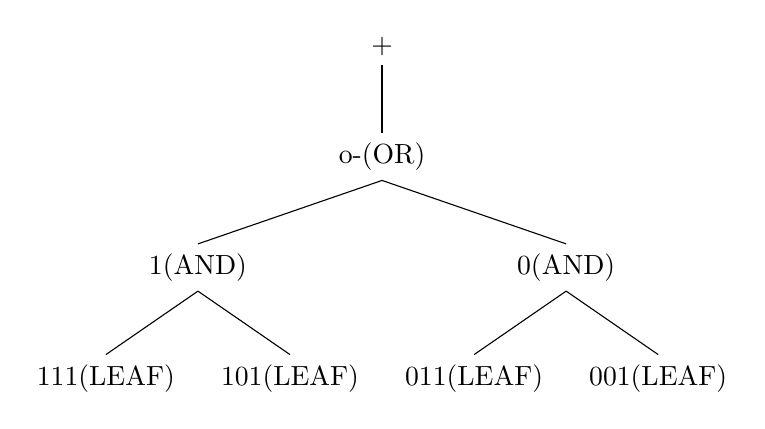
\begin{tikzpicture}
\tikzset{level distance=40pt, sibling distance=10pt}

\Tree
[.+
    [.o-(OR)
        [.1(AND)
            [.111(LEAF) ]
            [.101(LEAF) ]
        ]
        [.0(AND)
            [.011(LEAF) ]
            [.001(LEAF) ]
        ]
    ]
]

\end{tikzpicture}
\end{center}

A construção da árvore é realizada pela função \texttt{\_build} que utiliza uma fila \texttt{Queue} conforme especificado no algoritmo 3. Cada nó interno recebe uma valoração incompleta e uma função AND, associada ao operador universal, ou OR, associada ao operador existencial. Cada folha possui uma \texttt{substring} completa e uma valoração \texttt{flag} obtida por meio da função \texttt{evaluate\_expression}.

Após a construção da árvore, é realizado um percurso pós-fixo para criar uma pilha de \texttt{NodeT} na função \texttt{\_traversal\_stack} permitindo assim a avaliação da expressão codificada na árvore. O percurso pós-fixo e a pilha posfix estão detalhados no algoritmo 4. A última etapa consiste em desempilhar os nós da pilha posfix, conforme indicado no algoritmo 5, para obter o nó resultado por meio da função \texttt{solve}. O nó resultado contém tanto a flag booleana que indica a satisfabilidade como a string que representa o conjunto de soluções possíveis no caso de satisfabilidade.

O problema da satisfabilidade é mais complexo que o anterior e a abordagem escolhida para solucioná-lo incorpora o algoritmo de avaliar expressões booleanas. A ideia em alto nível é utilizar uma árvore binária (\texttt{class Tree}) que varre todas as possiblidades de valoração das variáveis, que estão codificadas pelos operadores $\exists$ e $\forall$. Os Nós \texttt{struct NodeT} da árvore de satisfabilidade têm como atributos uma \texttt{std::string substring}, indicando uma valoração possível, uma função \texttt{Function function}, que pode ser \texttt{AND, OR, LEAF} e uma valor booleano \texttt{bool flag}. Além dos ponteiros entre nós.

A árvore é construída através da função \texttt{\_build} que utiliza uma \texttt{Queue} como especificado em algorithm 3. Cada Nó interno recebe uma valoração incompleta e uma função AND, associada ao opearador quaulquer,  ou OR, associada ao operador existe. Cada folha tem uma \texttt{substring} completa e recebe uma valoração \texttt{flag}, através da função \texttt{evaluate\_expression}. Observe a árvore abaixo que representa o exemplo na expressão (1):

Uma vez construída a árvore booleana utilizamos um caminhamento posfix para construção de uma pilha de NodeT, na função \texttt{\_traversal\_stack}, que permite a avaliação da expressão codificada na árvore. O caminhamento posfix e a pilha de avaliaçaão estão contemplados no algoritmo 4. A última etapa consiste em retirar o nós da pilha de avalaicao, seguindo o algoritimo 5, a fim de se obeter o nó resultado, função \texttt{solve}. O nó resultado contém tanto a flag booleana indicando satisfabilidade ou não, como a string que inidica o pool de soluções possíveis no caso de satisfabilidade.

\textbf{Estruturas de Dados II}: 4 \texttt{Stack\textless NodeT*\textgreater}, 1 \texttt{Queue\textless NodeT*\textgreater}, 1 \texttt{Tree<NodeT*>}


\begin{adjustwidth}{1em}{1em}
\begin{algorithm}
\caption{Converter expressão lógica infixa para pós-fixa}
\begin{enumerate}
    \item Inicialize uma string vazia chamada $\text{{posfix\_formula}}$ para armazenar a fórmula pós-fixa.
    \item Crie uma pilha chamada $\text{{stack}}$ para auxiliar na conversão.
    \item Substitua quaisquer variáveis na fórmula infixa pelos valores correspondentes fornecidos na sequência $\text{{valuation}}$.
    \item Percorra cada caractere da fórmula infixa da esquerda para a direita.
    \item Para cada caractere:
    \begin{enumerate}
        \item Se for um valor booleano '0' ou '1', adicione-o à $\text{{posfix\_formula}}$.
        \item Se for um parêntese aberto '(', empilhe-o na pilha $\text{{stack}}$.
        \item Se for um parêntese fechado ')', desempilhe operadores da pilha $\text{{stack}}$ e adicione-os à $\text{{posfix\_formula}}$ até encontrar um parêntese aberto correspondente.
        \item Se for um operador (como AND, OR), enquanto houver operadores na pilha $\text{{stack}}$ com maior precedência ou a mesma precedência (e associatividade à esquerda), desempilhe-os e adicione à $\text{{posfix\_formula}}$. Em seguida, empilhe o operador atual na pilha $\text{{stack}}$.
    \end{enumerate}
    \item Após percorrer toda a fórmula infixa, desempilhe quaisquer operadores restantes da pilha $\text{{stack}}$ e adicione-os à $\text{{posfix\_formula}}$.
    \item A $\text{{posfix\_formula}}$ agora contém a expressão no formato pós-fixo.
    \item Retorne a $\text{{posfix\_formula}}$.
\end{enumerate}
\end{algorithm}


\begin{algorithm}
\caption{Avaliar expressão lógica pós-fixa com valores 0's e 1's}
\begin{enumerate}
    \item Chame a função $\text{{to\_posfix}}$ para converter a fórmula da sua forma infixa para a forma pós-fixa, aplicando a sequência de valores $\text{{valuation}}$ quando necessário.
    \item Inicialize uma pilha chamada $\text{{stack}}$ para armazenar temporariamente os valores da expressão.
    \item Percorra a $\text{{formula}}$ no formato pós-fixo da esquerda para a direita.
    \item Para cada caractere:
    \begin{enumerate}
        \item Se for um dígito '0' ou '1', empilhe o valor na pilha $\text{{stack}}$.
        \item Se for o operador '~' (NOT), desempilhe um valor da pilha, negue-o e empilhe o resultado na pilha $\text{{stack}}$.
        \item Se for um operador binário (AND ou OR), desempilhe dois valores da pilha, aplique a operação apropriada e empilhe o resultado na pilha $\text{{stack}}$.
    \end{enumerate}
    \item Após percorrer toda a expressão, o valor resultante estará no topo da pilha $\text{{stack}}$.
    \item Verifique se o valor no topo da pilha é '1'. Se for, retorne \text{{true}}, indicando que a expressão é verdadeira. Caso contrário, retorne \text{{false}}, indicando que a expressão é falsa.
\end{enumerate}
\end{algorithm}


\begin{algorithm}
\caption{Construção de uma Árvore de Expressões Lógicas usando uma Fila}
\begin{enumerate}
    \item Inicialize o nó raiz da árvore como nulo.
    \item Verifique se a profundidade (\textit{depth}) é igual a 1.
        \begin{enumerate}
            \item Se for igual a 1, crie um nó folha com o valor da avaliação da fórmula (\textit{formula}) e atribua-o como o nó raiz.
        \end{enumerate}
    \item Caso contrário, continue com a construção da árvore:
        \begin{enumerate}
            \item Inicialize um índice como 0.
            \item Use uma função (\textit{\_find\_operator}) para encontrar o próximo operador e seus operandos na avaliação (\textit{valuation}) com base no índice atual.
            \item Crie o nó raiz da árvore com o operador e a subexpressão obtidos da função anterior.
            \item Inicialize uma fila (queue) vazia para gerenciar os nós da árvore.
            \item Adicione o nó raiz à fila (queue).
        \end{enumerate}
    \item Execute um loop até que o operador encontrado seja um operador folha:
        \begin{enumerate}
            \item Obtenha o próximo operador e seus operandos da avaliação.
            \item Calcule o tamanho atual da fila (queue).
            \item Para cada nó na fila (queue) neste momento:
                \begin{enumerate}
                    \item Remova um nó da fila (queue) e defina-o como o nó atual (\textit{current}).
                    \item Crie dois nós filhos: left e right, anexando substring do parent concatenada com "1" ou "0", concatenada com a substring corrente.
                    \item Se o operador encontrado é um operador folha, avalie os valores dos nós filhos usando a função (\textit{evaluate\_expression}) e atribua os resultados aos campos \textit{flag} dos nós.
                    \item Adicione os nós filhos à fila (queue).
                \end{enumerate}
        \end{enumerate}
    \item Após a conclusão do loop, a árvore estará construída.
\end{enumerate}
\end{algorithm}




\begin{algorithm}
\caption{Avaliação a partir da Pilha Pós-Fixa}
\begin{enumerate}
    \item Inicie com duas pilhas vazias: uma para a pilha de nós e outra para a pilha de travessia.
    \item Comece a travessia a partir da raiz da árvore.
    \item Enquanto houver nós para serem explorados ou a pilha de nós não estiver vazia:
    \begin{enumerate}
        \item Se o nó atual não for nulo:
        \begin{enumerate}
            \item Empilhe o nó na pilha de nós e na pilha de travessia.
            \item Avance para o filho direito do nó atual, se existir, e continue a partir desse ponto.
        \end{enumerate}
        \item Caso contrário:
        \begin{enumerate}
            \item Desempilhe um nó da pilha de nós e vá para o seu filho esquerdo, se existir.
        \end{enumerate}
    \end{enumerate}
\end{enumerate}
\end{algorithm}




\begin{algorithm}
\caption{Avaliação a partir da pilha posfix}
\begin{enumerate}
    \item Inicie a pilha de avaliação como vazia.
    \item Enquanto a pilha de travessia (\texttt{traversal\_stack}) não estiver vazia, faça o seguinte:
    \begin{enumerate}
        \item Retire o nó do topo da pilha de travessia.
        \item Se o nó for uma folha (um operando), adicione-o à pilha de avaliação.
        \item Se o nó for um operador, desempilhe os operandos necessários da pilha de avaliação, aplique a operação representada pelo operador e coloque o resultado na pilha de avaliação.
    \end{enumerate}
    \item Após avaliar todos os nós da pilha de travessia, a pilha de avaliação conterá o resultado final da expressão da árvore.
    \item Realize as ações desejadas com base no resultado da avaliação, como imprimir, armazenar ou executar operações adicionais.
\end{enumerate}
\end{algorithm}

\end{adjustwidth}


\section{Análise de Complexidade}
Essa seção se dedica a analisar a complexidade assintótica, em termos de espaço e de tempo, das principais funções envolvidas nos problemas de Expressões booleanas e Satisfabilidade.

% Vou analisar a complexidade de tempo das duas funções set_values e to_posfix em termos do número de caracteres na entrada (len), assumindo que as funções auxiliares is_digit, is_operand, precedence, Stack::add, Stack::peek, e Stack::pop têm complexidade constante O(1).

\subsection{set\_values}
O loop for itera sobre cada caractere na fórmula fazendo operações simples.
A verificação de espaço em branco com \texttt{std::isspace(c)} é uma operação constante \texttt{O(1)}.
Quando um dígito é encontrado, há um loop do-while que percorre a sequência de dígitos, mas isso é feito apenas uma vez para cada dígito na entrada, portanto, ainda é uma operação \texttt{O(1)} para cada dígito.
No geral, o loop for é executado uma vez para cada caractere na entrada, o que resulta em uma complexidade de tempo de $O(n)$, onde $n$ é o comprimento da fórmula.

\subsection{to\_posfix}
A função \texttt{set\_values} é chamada primeiro, que tem uma complexidade de tempo de \texttt{O(n)}.
A função principal percorre a fórmula infixa e, para cada caractere, executa operações no topo da pilha.
As operações principais dentro do loop incluem a adição de caracteres à string posfix\_formula e operações na pilha.
Para caracteres como '0' e '1', a operação é \texttt{O(1)}).
Para os parênteses \texttt{(}, \texttt{)}, e operandos, as operações de empilhamento e desempilhamento na pilha podem ser \texttt{O(1)} em média, pois o número de elementos na pilha é limitado.
No geral, o loop for é executado uma vez para cada caractere na entrada, resultando em uma complexidade de tempo de \texttt{O(n)}, onde \texttt{n} é o comprimento da fórmula.


\subsection{boolean\_evaluation}
A função \texttt{to\_posfix} é chamada primeiro e tem uma complexidade de tempo de \texttt{O(n)}, como discutido anteriormente.
O loop for itera sobre cada caractere na fórmula de entrada. Para cada caractere, as seguintes operações são executadas:
A verificação de \texttt{is\_digit(c)} é uma operação \texttt{O(1)}.
Para o caractere \texttt{~}, uma operação \texttt{\_neg} é realizada em um único caractere, o que é O(1).
Para os operadores \& e $|$, duas operações \texttt{\_and} ou \texttt{\_or} são realizadas em dois caracteres, resultando em \texttt{O(1)}.
Portanto, para cada caractere na fórmula de entrada, as operações dentro do loop são realizadas em tempo constante \texttt{O(1)}.

No geral, o loop for é executado uma vez para cada caractere na fórmula, resultando em uma complexidade de tempo total de \texttt{O(n)}, onde \texttt{n} é o comprimento da fórmula de entrada.

\subsection{Tree::\_build}
\begin{itemize}
  \item \textbf{Complexidade de Tempo da Função \_build}:
    \begin{enumerate}
      \item Se a profundidade \_depth da árvore for igual a 1, a função cria um único nó \_root. Isso envolve uma chamada para evaluate\_expression, que tem uma complexidade de tempo de \texttt{O(n)} (onde n é o comprimento da fórmula). Portanto, a complexidade de tempo neste caso é \texttt{O(n)}.
      \item Caso contrário, a função começa a construir a árvore de maneira iterativa usando um loop. A cada iteração do loop, a função chama \_find\_operator, que tem uma complexidade de tempo de O(1) para encontrar o próximo operador na fórmula. Em seguida, ela cria dois nós filhos para o nó atual em cada iteração.
      \item Para cada folha criado, é necessário avaliar a expressão usando evaluate\_expression. O número de folhas será dado por \texttt{2ˆ\_depth}, que corresponde ao número total de chamadas para evaluate\_expression ao longo do processo.
      \item Portanto, a complexidade de tempo geral da função \_build é dominada pelo número de chamadas para evaluate\_expression, logo temos custo exponencial \texttt{O(2ˆn)}.
    \end{enumerate}
  \item \textbf{Complexidade de Espaço da Função \_build}:
    \begin{enumerate}
      \item Para cada nó criado na árvore, a função aloca memória para armazenar informações sobre o nó, como sua valuation, sub\_string, função e outros atributos. Portanto, a complexidade de espaço está relacionada ao número total de nós na árvore.
      \item Além disso, a função utiliza uma fila (representada como \texttt{Queue\textless char\textgreater}queue) para gerenciar os nós à medida que a árvore é construída. A quantidade de espaço necessário para manter a fila é proporcional ao número de nós presentes na árvore.
      \item Portanto, a complexidade de espaço da função \_build está relacionada ao número de nós na árvore, que pode ser substancial, especialmente para árvores profundas.
    \end{enumerate}
\end{itemize}


\subsection{Tree::\_traversal\_stack}
\begin{itemize}
  \item \textbf{Complexidade de Tempo da Função \_traversal\_stack}:
    \begin{enumerate}
      \item A função realiza uma travessia pós-ordem na árvore. Ela utiliza duas pilhas, node\_stack e traversal\_stack, para realizar a travessia.
      \item O loop while executa enquanto o nó atual não for nulo ou a pilha node\_stack não estiver vazia. Dentro do loop, as operações principais incluem adicionar e remover nós das pilhas.
      \item Quando o nó atual não é nulo, ele é adicionado às duas pilhas, e o algoritmo avança para o filho direito do nó atual. Essa operação envolve operações de empilhamento e desempilhamento, mas são executadas em tempo constante, O(1).
      \item Quando o nó atual é nulo, um nó é desempilhado da pilha node\_stack, e o algoritmo avança para o filho esquerdo desse nó. Novamente, envolve operações de empilhamento e desempilhamento em pilhas, mas em tempo constante O(1).
      \item Portanto, para cada nó na árvore, há operações de empilhamento e desempilhamento, que são executadas em tempo constante O(1). Como o loop while executa para cada nó na árvore uma vez, a complexidade de tempo da função \_traversal\_stack é O(n), onde n é o número de nós na árvore. 
    \end{enumerate}
  \item \textbf{Complexidade de Espaço da Função \_traversal\_stack}:
    \begin{enumerate}
      \item A função utiliza duas pilhas, node\_stack e traversal\_stack, para gerenciar os nós durante a travessia. A quantidade de espaço necessário para manter essas pilhas depende do número de nós na árvore.
      \item Como mencionado anteriormente, a complexidade de tempo da função é O(n), onde n é o número de nós na árvore. Portanto, o espaço necessário para as pilhas é proporcional ao número de nós na árvore.
      \item No pior caso, a árvore pode ter n nós, o que resultaria em um espaço adicional de O(n) para as pilhas.

    \end{enumerate}
\end{itemize}

\subsection{Tree::solve}
\begin{itemize}
  \item \textbf{Complexidade de Tempo da Função solve}:
    \begin{enumerate}
      \item A função solve é responsável por resolver a árvore de expressões lógicas que já foi construída. Ela utiliza duas pilhas, stack\_evaluation e post\_stack, durante o processo de avaliação.
      \item A função inicia recuperando a pilha post\_stack com a travessia pós-ordem da árvore, o que envolve um custo de tempo de O(n), onde n é o número de nós na árvore.
      \item Em seguida, ela inicia um loop while que percorre os nós da pilha post\_stack.
      \item No loop while, a função realiza operações que envolvem adicionar e remover nós das pilhas stack\_evaluation e post\_stack, bem como avaliar expressões, executar operações lógicas, atualizar flags e valuations dos nós.
      \item A operação de adicionar e remover nós das pilhas é executada em tempo constante O(1).
      \item A avaliação de expressões, execução de operações lógicas e atualizações nos nós também são realizadas em tempo constante O(1).
      \item O loop while é executado para cada nó na pilha post\_stack, que é diretamente proporcional ao número de nós na árvore.
      \item Portanto, a complexidade de tempo da função solve é dominada pelo loop while e é O(n), onde n é o número de nós na árvore.
    \end{enumerate}
  \item \textbf{Complexidade de Espaço da Função solve}:
    \begin{enumerate}
      \item A função solve utiliza duas pilhas, stack\_evaluation e post\_stack, para gerenciar os nós durante o processo de avaliação.
      \item A quantidade de espaço necessário para manter essas pilhas é proporcional ao número de nós na árvore.
      \item Como mencionado anteriormente, a complexidade de tempo da função é O(n), onde n é o número de nós na árvore. Portanto, o espaço necessário para as pilhas é proporcional ao número de nós na árvore.
      \item No pior caso, a árvore pode ter n nós, o que resultaria em um espaço adicional de O(n) para as pilhas.
    \end{enumerate}
\end{itemize}

\section{Estratégias de Robustez}
Com o objetivo de tornar o programa mais robusto e evitar problemas com entradas inválidas, foram implementadas verificações nos inputs do terminal no arquivo \texttt{main.cpp}. Isso garante que o usuário não insira opções inválidas e, caso o faça, o programa apresenta uma mensagem de erro no terminal e encerra a execução.

Além disso, foram criadas classes de exceção, como \texttt{ExceptionEmptyStack} e \texttt{ExceptionEmptyQueue}. Nas funções de remoção das respectivas estruturas de dados, lançamos essas exceções caso a estrutura esteja vazia. Isso permite um tratamento adequado de situações excepcionais, garantindo a integridade do programa.

Entretanto, é importante destacar que o programa ainda possui limitações, uma vez que não cobre um amplo espectro de possíveis entradas de dados, presumindo que o usuário fornecerá entradas corretas. As verificações se concentram principalmente na detecção de opções inválidas.

Para manter a integridade do programa e evitar vazamentos de memória, todos os Tipos Abstratos de Dados (TADs) implementam destrutores apropriados. Além disso, foram realizados testes com o Valgrind, e nenhum erro relacionado à alocação de memória foi observado.

\section{Conclusões}

\end{document}
